\documentclass[polish, 11pt, a4paper]{article}

\usepackage[autostyle]{csquotes}
\DeclareQuoteAlias{dutch}{polish}
\usepackage[T1]{fontenc}
\usepackage{geometry}
\geometry{
	a4paper,
	total={170mm,257mm},
	left=25mm,
	right=25mm,
	top=20mm,
}
\usepackage{polski}
\usepackage[utf8]{inputenc}
\usepackage{babel}
\usepackage{microtype}
\usepackage{lmodern}
\usepackage{multirow}
\usepackage{amsmath}
\usepackage{caption}
\usepackage{graphicx}
\usepackage{graphics}
\usepackage{float}
\usepackage{enumitem}
\usepackage{ragged2e}
\usepackage{parskip}
\RaggedRightParindent = 24 pt
\usepackage{indentfirst}
\usepackage[figurename=Wykres]{caption}

\begin{document}
	\begin{titlepage}
	\centering
	\Huge Laboratorium Podstaw Fizyki\\
	\vspace{1cm}
	\huge Ćwiczenie 81B \enquote{Wyznaczanie promienia krzywizny soczewki i długości fali świetlnej za pomocą pierścieni Newtona}\\
	\vspace{1cm}
	\raggedright
	\huge Prowadzący: mgr Karolina Paradowska\\
	\vspace{.5cm}
	\begin{table}[h]
		\centering
		\resizebox{\columnwidth}{!}{%
		\begin{tabular}{|r|l|}\hline
			Imię i Nazwisko	&Marcin Kotas\\\hline
			Nr indeksu		&235098\\\hline
			Wydział			&Elektroniki\\\hline
			Termin zajęć	&24.10.2017, godz. 9.15\\\hline
			Numer grupy ćwiczeniowej&5\\\hline
			Data oddania sprawozdania&31.10.2017\\\hline
		\end{tabular}%
		}
	\end{table}
	\end{titlepage}
	\section{Wstęp teoretyczny}
		\RaggedRight
		%\raggedright
		Pierścienie Newtona to zjawisko, które powstaje w wyniku interferencji fal światła. Ukazuje się w postaci naprzemiennych okręgów jasnych i ciemnych pól. Takie okręgi po raz pierwszy zauważył Newton (dlatego noszą nazwę pierścieni Newtona), a poprawnie zostały opisane przez Hooke’a w 1664 roku. Charakterystyczny wzór uzyskuje się poprzez położenie płasko-wypukłej soczewki (stroną wypukłą w dół) na płaskim szkle. W ten sposób szkła stykają się tylko w samym środku. Wszędzie dookoła jest przerwa między szkłami, która stopniowo zwiększa się z odległością od środka. Na tak ustawioną soczewkę pada z góry światło monochromatyczne, które odbija się zarówno od wypukłej ściany soczewki, jak i od płaskiego szkła pod nią. Jednocześnie przy przechodzeniu między ośrodkami (szkło-powietrze) promienie ulegają załamaniu. Te dwa promienie nakładają się na siebie tworząc zjawisko interferencji. W zależności od przebytej drogi fale będą się wzmacniać lub wygaszać według następujących zasad:\\
		\begin{itemize}
			\item Wzmocnienie nastąpi w miejscach, gdzie różnica przebytej drogi będzie równa wielokrotności długości fali (grzbiety i dna funkcji będą w tych samych miejscach). W takim wypadku fale będą w tej samej fazie, więc amplitudy się dodadzą. W rezultacie obserwowany obszar będzie jasny. (\(\Delta L=n\cdot\lambda\))
			\item Wygaszenie nastąpi w miejscach, gdzie różnica przebytej drogi będzie równa nieparzystej wielokrotności połowy długości fali (grzbiety jednej fali spotkają się z dnami drugiej fali). W takim wypadku fale będą w przeciwnych fazach (przesunięte o \(180^{\circ}\) ), a więc się wygaszą. W rezultacie obserwowany obszar będzie ciemny. (\(\Delta L = (2n+1)\cdot\frac{\lambda}{2}\))
		\end{itemize}
		Ponieważ soczewka jest okrągła, w wyniku interferencji powstają charakterystyczne jasne i ciemne prążki wokół środka soczewki. W miarę wzrostu odległości od środka kolejne prążki coraz bardziej się zagęszczają, aż przestają być rozróżnialne. Spowodowane jest co coraz większą przerwą między soczewką, a szklaną płytką. Na samym środku ukazuje się ciemny obszar, ponieważ w chwili odbicia fali od dolnego płaskiego szkła następuje odwrócenie fali, przez co jest przesunięta o \(180^{\circ}\). Jeśli użyte zostanie białe światło to powstają kolorowe prążki (fale o różnych długościach są załamywane w różnym stopniu)
		
		Efekt ten jest wykorzystywany w badaniu jakości powierzchni optycznych ze względu na bardzo wysoką dokładność. Rozmiary promieni mogą posłużyć w wyznaczaniu promienia krzywizny analizowanych powierzchni, a zniekształcenie pierścieni określa inne właściwości, jak odstępstwa od regularnego kształtu. W przemyśle zjawisko to jest wykorzystywane przy badaniu jakości szkieł w obiektywach.
		Możliwe jest również wyznaczenie współczynnika załamania światła cieczy znajdującej się pomiędzy soczewką, a płaskim szkłem.
		
		Celem ćwiczenia było zapoznanie się ze zjawiskiem interferencji światła występującym w klinie optycznym oraz obliczenie promienia krzywizny soczewki na podstawie promieni pierścieni Newtona, korzystając ze wzoru: 
		\begin{displaymath}
		R=\frac{r^2}{k\cdot \lambda}
		\end{displaymath}
		W tym celu użyta została lampa z filtrem interferencyjnym 600nm, mikroskop z czujnikiem zegarowym, soczewka płasko-wypukła oraz szklana płytka płasko-równoległa. Zostały zmierzone promienie 5 pierścieni, zaczynając od prążka rzędu 7. Aby zwiększyć dokładność pomiarów każdy pomiar został przeprowadzony 10 razy. Zmierzono również grubość każdego prążka, która użyta została przy wyznaczeniu błędu eksperymentatora.
		
	\newpage
	\section{Wyniki pomiarów}
	
	\subsection{Wykonanie pomiarów}
		Aby zmierzyć promień prążka wykonane zostały pomiary współrzędnej jego lewej oraz prawej krawędzi. Przeprowadzono takie same pomiary dla prążków o rzędach 7-11, przybierając za prążek rzędu 0 ciemny środek obrazu. Każdy pomiar został powtórzony 10 razy, dając w sumie 100 pomiarów. Zostały one przedstawione w tabelach 1-5. Na koniec zmierzono raz grubość każdego z obserwowanych prążków, której połowę przyjęto za błąd eksperymentatora. Grubość \textbf{\textit{d}} została podana w podpisach tabel.
	\subsection{Obliczenia}
	\subsubsection{Opracowanie wyników}
		Dla każdej z wyliczonych współrzędnych została obliczona wartość średnia.
		Ten, oraz następne przykładowe obliczenia przedstawiają przypadek lewej współrzędnej pierścienia nr 7:
		\begin{displaymath}
		\bar{a_l}=\frac{1}{10}\sum_{i=1}^{10}a_{li}=\frac{1}{10}(6,24+6,23+\dots+6,23+6,22)=\frac{1}{10}\cdot 62,31=6,231 [mm]
		\end{displaymath}
		Następnie wyliczona została niepewność typu A dla wszystkich współrzędnych:\\
		\begin{align*}
		u_A(a_l)&=\sqrt{\frac{\sum_{i=1}^{10} (a_{li}-\bar{a_l})^2}{10(10-1)}}\\
				&=\sqrt{\frac{(6,24-6,231)^2+(6,23-6,231)^2+\dots+(6,22-6,231)^2}{90}}\\
				&=0,001795055\approx 0,0018 [mm]
		\end{align*}\\
		Na niepewność standardową typu B składają się niepewność czujnika zegarowego \(\Delta{_px}\) oraz niepewność eksperymentatora (w tym przypadku równej połowie grubości pierścienia \(\Delta{_ex}=\frac{d}{2}\)):
		\begin{align*}
		u_B(a_l)	&=\sqrt{\frac{(\Delta{_pa_l})^2}{3}+\frac{(\Delta{_ea_l})^2}{3}}=\sqrt{\frac{0,01^2}{3}+\frac{0,02^2}{3}}\\
					&=0,012909944\approx 0,0129[mm]
		\end{align*}
		Finalna niepewność standardowa całkowita wynosi:
		\begin{align*}
		u(a_l)	&=\sqrt{u_A^2(a_l)+u_B^2(a_l)}=\sqrt{0,0018^2+0,0129^2}\\
				&=0,013034143\approx 0,014[mm]
		\end{align*}
		Średni promień \(r\) został obliczony jako średnia z różnic współrzędnych podzielonych przez 2:
		\begin{align*}
		\bar{r}	&=\frac{1}{10}\sum_{i=1}^{10}\frac{1}{2}|a_{li}-a_{bi}|\\
				&=\frac{1}{20}(|6,24-3,04|+|6,23-3,04|+\dots+|6,22-3,05|)\\
				&=1,5915\approx 1,592[mm]
		\end{align*}
		Dokładność promienia jest równa mniejszej dokładności współrzędnych
		(w tym przypadku obie współrzędne określone są z taką samą dokładnością):
		\begin{displaymath}
		u(r)=u(a_l)=u(a_p)=0,014[mm]
		\end{displaymath}
	\subsubsection{Wyznaczanie promienia krzywizny soczewki}
		Promień krzywizny wyznacza się z wyrażenia \(R=\frac{r^2}{k\cdot \lambda}\), przy czym \(k\) jest numerem badanego prążka, \(\lambda\) długością fali światła.
		Promień krzywizny został wyznaczony dla każdego pierścienia, z użyciem uśrednionych wartości promieni pierścieni (Wyniki wszystkich obliczeń przedstawione są w Tabeli 6):\\
		\begin{displaymath}
		R=\frac{r^2}{k\cdot \lambda}=\frac{(1,592\cdot 10^{-3})^2}{7\cdot 600\cdot 10^{-9}}\approx 0,603065[m]
		\end{displaymath}\\
		Pomiar promienia krzywizny soczewki jest pomiarem pośrednim, więc jego niepewność jest niepewnością złożoną:
		\begin{align*}
		u_c(R)	&=\sqrt{\left(\frac{\partial R}{\partial r}\right)^2\cdot u^2(r)+\left(\frac{\partial R}{\partial \lambda}\right)^2\cdot u^2(\lambda)}\\
				&=\sqrt{\left(\frac{2r}{k\cdot \lambda}\right)^2\cdot u^2(r) + \left(-\frac{r^2}{k\cdot \lambda^2}\right)^2\cdot u^2(\lambda)}\\
				&=\sqrt{
					\begin{aligned}
					&\left(\frac{2\cdot 1,592\cdot 10^{-3}}{7\cdot 600\cdot 10^{-9}}\right)^2\cdot (0,014\cdot 10^{-3})^2\\ &+\left(-\frac{(1,592\cdot 10^{-3})^2}{7\cdot (600\cdot 10^{-9})^2}\right)^2\cdot (5,7735\cdot 10^{-9})^2
					\end{aligned}
				} \approx 0,012093[m]
		\end{align*}\\
		Na koniec należy wyliczyć średni promień krzywizny soczewki w sposób analogiczny do liczenia średniej wartości współrzędnej:
		\begin{displaymath}
			\bar{R}=0,6041[m]
		\end{displaymath}\\
		Niepewność wartości średniej została wyznaczona poprzez obliczenie wartości odchylenia standardowego średniej:
		\begin{displaymath}
			u(R)=\sqrt{\frac{\sum_{i=1}^{5}(R_i-\bar{R})^2}{5-1}}=0,001033893\approx 0,0011[m]
		\end{displaymath}
		
		Promień krzywizny soczewki można również otrzymać korzystając z regresji liniowej (Wykres 1). Otrzymany w ten sposób promień wynosi:
		\begin{displaymath}
		R=0,6061 [m]
		\end{displaymath}
		
		Aby wyznaczyć niepewność szukanego w ten sposób promienia krzywizny w programie Excel, należy skorzystać z funkcji REGLINP. Otrzymana niepewność wynosi:
		\begin{displaymath}
		u(R)=0,003186879\approx 0,0032[m]
		\end{displaymath}
		
	\newpage
	\subsection{Tabele i wykresy}
		\begin{table}[H]
		\begin{minipage}{.5\textwidth}
			\centering
			\captionsetup{singlelinecheck=false, margin = .5cm, justification=centering}
			\caption{Wyniki pomiarów dla k = 7\newline 	d = 0,04 mm}
			\begin{tabular}{|r|c|c|c|} \hline
					&	\textit{a\textsubscript{l}}	&	\textit{a\textsubscript{p}}	&	\textit{r}	\\
				&&& \\[-1em]
				\textit{Lp.}& \(\times{10^{-3} [m]}\)& \(\times{10^{-3} [m]}\)& \(\times{10^{-3} [m]}\) \\\hline	
				1	&	6,24	&	3,04	&	1,60	\\\hline
				2	&	6,23	&	3,04	&	1,60	\\\hline
				3	&	6,24	&	3,05	&	1,60	\\\hline
				4	&	6,23	&	3,05	&	1,59	\\\hline
				5	&	6,23	&	3,05	&	1,59	\\\hline
				6	&	6,23	&	3,05	&	1,59	\\\hline
				7	&	6,23	&	3,06	&	1,59	\\\hline
				8	&	6,23	&	3,04	&	1,60	\\\hline
				9	&	6,23	&	3,05	&	1,59	\\\hline
				10	&	6,22	&	3,05	&	1,59	\\\hline
				\(\Delta{_px}\)	&	0,01	&	0,01	&		\\\hline
				\(\bar{x}\)	&	6,231	&	3,048	&	1,592	\\\hline
				\(u_A(x)\)	&	0,0018	&	0,002	&		\\\hline
				\(u_B(x)\)	&	0,0129	&	0,0129	&		\\\hline
				\(u(x)\)	&	0,013034	&	0,013064	&		\\\hline
				\(\approx{u(x)}\)	&	0,014	&	0,014	&	0,014	\\\hline
			\end{tabular}
			\vspace{0.75cm}
			
			\caption{Wyniki pomiarów dla k = 8 \newline d = 0,04 mm}
			\begin{tabular}{|r|c|c|c|} \hline
					&	\textit{a\textsubscript{l}}	&	\textit{a\textsubscript{p}}	&	\textit{r}	\\
				&&& \\[-1em]
				\textit{Lp.}& \(\times{10^{-3} [m]}\)& \(\times{10^{-3} [m]}\)& \(\times{10^{-3} [m]}\) \\\hline
				1	&	6,34	&	2,93	&	1,71	\\\hline
				2	&	6,34	&	2,94	&	1,70	\\\hline
				3	&	6,34	&	2,93	&	1,71	\\\hline
				4	&	6,35	&	2,94	&	1,71	\\\hline
				5	&	6,34	&	2,93	&	1,71	\\\hline
				6	&	6,34	&	2,94	&	1,70	\\\hline
				7	&	6,35	&	2,93	&	1,71	\\\hline
				8	&	6,34	&	2,93	&	1,71	\\\hline
				9	&	6,34	&	2,93	&	1,71	\\\hline
				10	&	6,34	&	2,93	&	1,71	\\\hline
				\(\Delta{_px}\)	&	0,01	&	0,01	&		\\\hline
				\(\bar{x}\)	&	6,342	&	2,933	&	1,705	\\\hline
				\(u_A(x)\)	&	0,0013	&	0,0015	&		\\\hline
				\(u_B(x)\)	&	0,0129	&	0,0129	&		\\\hline
				\(u(x)\)	&	0,012979	&	0,013	&		\\\hline
				\(\approx{u(x)}\)	&	0,013	&	0,013	&	0,013	\\\hline
			\end{tabular}
		
		\end{minipage}%
		\begin{minipage}{.5\textwidth}
			\centering
			\captionsetup{singlelinecheck=false, margin = .5cm, justification=centering}
			\caption{Wyniki pomiarów dla k = 9 \newline d = 0,03 mm}
			\begin{tabular}{|r|c|c|c|} \hline
					&	\textit{a\textsubscript{l}}	&	\textit{a\textsubscript{p}}	&	\textit{r}	\\
				&&& \\[-1em]
				\textit{Lp.}& \(\times{10^{-3} [m]}\)& \(\times{10^{-3} [m]}\)& \(\times{10^{-3} [m]}\) \\\hline
				1	&	6,46	&	2,83	&	1,82	\\\hline
				2	&	6,44	&	2,84	&	1,80	\\\hline
				3	&	6,46	&	2,84	&	1,81	\\\hline
				4	&	6,44	&	2,84	&	1,80	\\\hline
				5	&	6,44	&	2,84	&	1,80	\\\hline
				6	&	6,45	&	2,84	&	1,81	\\\hline
				7	&	6,44	&	2,82	&	1,81	\\\hline
				8	&	6,45	&	2,83	&	1,81	\\\hline
				9	&	6,44	&	2,83	&	1,81	\\\hline
				10	&	6,44	&	2,83	&	1,81	\\\hline
				\(\Delta{_px}\)	&	0,01	&	0,01	&		\\\hline
				\(\bar{x}\)	&	6,446	&	2,834	&	1,806	\\\hline
				\(u_A(x)\)	&	0,0027	&	0,0022	&		\\\hline
				\(u_B(x)\)	&	0,0104	&	0,0104	&		\\\hline
				\(u(x)\)	&	0,010745	&	0,010641	&		\\\hline
				\(\approx{u(x)}\)	&	0,011	&	0,011	&	0,011	\\\hline
			\end{tabular}
			\vspace{0.75cm}

			\caption{Wyniki pomiarów dla k = 10 \newline d = 0,04 mm}
			\begin{tabular}{|r|c|c|c|} \hline
					&	\textit{a\textsubscript{l}}	&	\textit{a\textsubscript{p}}	&	\textit{r}	\\
				&&& \\[-1em]
				\textit{Lp.}& \(\times{10^{-3} [m]}\)& \(\times{10^{-3} [m]}\)& \(\times{10^{-3} [m]}\) \\\hline
				1	&	6,56	&	2,73	&	1,92	\\\hline
				2	&	6,54	&	2,74	&	1,90	\\\hline
				3	&	6,53	&	2,74	&	1,90	\\\hline
				4	&	6,54	&	2,73	&	1,91	\\\hline
				5	&	6,54	&	2,75	&	1,90	\\\hline
				6	&	6,53	&	2,73	&	1,90	\\\hline
				7	&	6,54	&	2,73	&	1,91	\\\hline
				8	&	6,54	&	2,73	&	1,91	\\\hline
				9	&	6,54	&	2,74	&	1,90	\\\hline
				10	&	6,54	&	2,73	&	1,91	\\\hline
				\(\Delta{_px}\)	&	0,01	&	0,01	&		\\\hline
				\(\bar{x}\)	&	6,540	&	2,735	&	1,903	\\\hline
				\(u_A(x)\)	&	0,0026	&	0,0022	&		\\\hline
				\(u_B(x)\)	&	0,0129	&	0,0129	&		\\\hline
				\(u(x)\)	&	0,013166	&	0,013102	&		\\\hline
				\(\approx{u(x)}\)	&	0,014	&	0,014	&	0,014	\\\hline
			\end{tabular}
		
			
		
		\end{minipage}
	
		\end{table}
	\newpage
		\begin{table}[h]
		\centering
		\captionsetup{singlelinecheck=false, margin = 4.5cm, justification=centering}
		\caption{Wyniki pomiarów dla k = 11 \newline d = 0,03 mm}
		\begin{tabular}{|r|c|c|c|} \hline
			&	\textit{a\textsubscript{l}}	&	\textit{a\textsubscript{p}}	&	\textit{r}	\\
			&&& \\[-1em]
			\textit{Lp.}& \(\times{10^{-3} [m]}\)& \(\times{10^{-3} [m]}\)& \(\times{10^{-3} [m]}\) \\\hline
			1	&	6,65	&	2,64	&	2,01	\\\hline
			2	&	6,65	&	2,65	&	2,00	\\\hline
			3	&	6,63	&	2,64	&	2,00	\\\hline
			4	&	6,64	&	2,64	&	2,00	\\\hline
			5	&	6,64	&	2,64	&	2,00	\\\hline
			6	&	6,64	&	2,65	&	2,00	\\\hline
			7	&	6,63	&	2,64	&	2,00	\\\hline
			8	&	6,64	&	2,64	&	2,00	\\\hline
			9	&	6,64	&	2,64	&	2,00	\\\hline
			10	&	6,63	&	2,64	&	2,00	\\\hline
			\(\Delta{_px}\)	&	0,01	&	0,01	&		\\\hline
			\(\bar{x}\)	&	6,639	&	2,642	&	1,999	\\\hline
			\(u_A(x)\)	&	0,0023	&	0,0013	&		\\\hline
			\(u_B(x)\)	&	0,0104	&	0,0104	&		\\\hline
			\(u(x)\)	&	0,010667	&	0,010493	&		\\\hline
			\(\approx{u(x)}\)	&	0,011	&	0,011	&	0,011	\\\hline
		\end{tabular}
		\vspace{0.75cm}
		
		\captionsetup{margin = 0cm}
		\caption{Wyznaczenie promienia krzywizny R}
		\begin{tabular}{|r|c|c|c|c|c|c|c|c|c|c|} \hline
			&&&&&&&&&& \\[-1em]
				&	\(\lambda\)	&	\(u(\lambda)\)	&	\(k\)	&	\(r\)	&	\(u(r)\)	&	\(R\)	&	\(u_c(R)\)	&	\(\bar{R}\)	&	\(u(R)\)	&	\(\approx u(R)\)	\\
			&&&&&&&&&& \\[-1em]
			 &\(\times{10^{-9}} \)&\(\times{10^{-9}} \)& &\(\times{10^{-3}} \)&\(\times{10^{-3}} \)&\multirow{2}{*}{\([m]\)}&\multirow{2}{*}{\([m]\)}&\multirow{2}{*}{\([m]\)}&\multirow{2}{*}{\([m]\)}&\multirow{2}{*}{\([m]\)}\\
			\textit{Lp.}	&	\([m]\)	&	\([m]\)	&		&	\([m]\)	&	\([m]\)	&	&	&	&	&	\\\hline
			1	&	\multirow{5}{*}{600}&	\multirow{5}{*}{5,7735}	&	7	&	1,592	&	0,014	&	0,603	&	0,013	&	\multirow{5}{*}{0,6041}	&	\multirow{5}{*}{0,001034}	&	\multirow{5}{*}{0,0011}	\\ \cline{1-1} \cline{4-8}
			2	&		&		&	8	&	1,705	&	0,013	&	0,605	&	0,011	&		&		&		\\ \cline{1-1} \cline{4-8}
			3	&		&		&	9	&	1,81	&	0,011	&	0,6040	&	0,0094	&		&		&		\\ \cline{1-1} \cline{4-8}
			4	&		&		&	10	&	1,903	&	0,014	&	0,603	&	0,011	&		&		&		\\ \cline{1-1} \cline{4-8}
			5	&		&		&	11	&	2,00	&	0,011	&	0,6052	&	0,0089	&		&		&		\\\hline
		\end{tabular}
		\end{table}
	%\vspace{.5cm}
		\begin{figure}[H]
			\centering
			\caption{Promień krzywizny soczewki - regresja liniowa}
			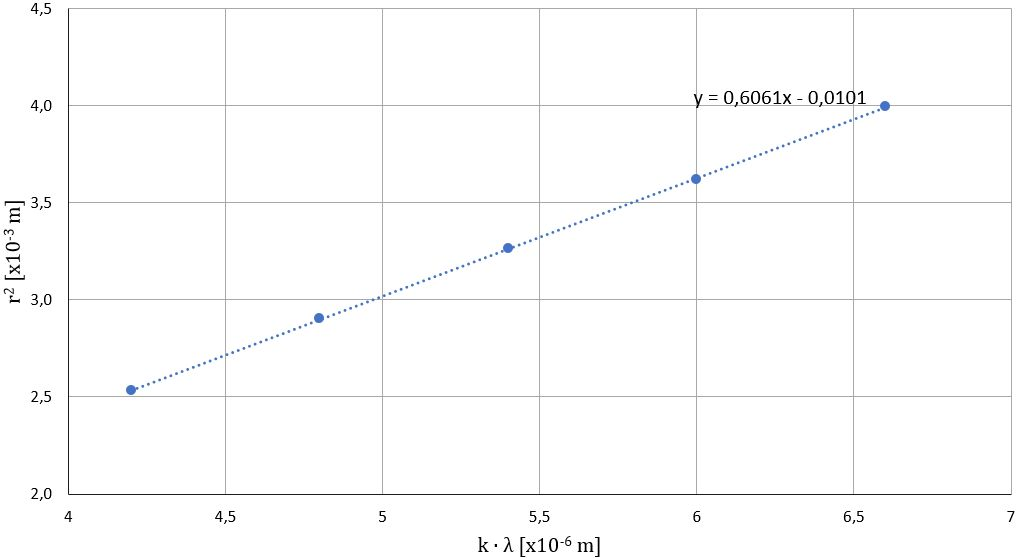
\includegraphics[width=.88\textwidth]{Fizyka81Wykres}
			\\
			\vspace{.1cm}
			\(R=0,6061[m]\) \hspace{1cm}\(u(R)=0,0032[m]\)
		\end{figure}
	
	%\newpage
	\section{Ostateczne wyniki}
		Ostateczne wyniki wraz z zaokrągleniami:
		\begin{description}[align=right,labelwidth=8cm]
			\item [Promień pierścienia rzędu 7:]{\((1,592\pm 0,014)\times{10^{-3}}m\)}
			\item [Promień pierścienia rzędu 8:]{\((1,705\pm 0,013)\times{10^{-3}}m\)}
			\item [Promień pierścienia rzędu 9:]{\((1,806\pm 0,011)\times{10^{-3}}m\)}
			\item [Promień pierścienia rzędu 10:]{\((1,903\pm 0,014)\times{10^{-3}}m\)}
			\item [Promień pierścienia rzędu 11:]{\((1,999\pm 0,011)\times{10^{-3}}m\)}
			\item [Promień R wyznaczony algebraicznie:]{\((0,6041\pm 0,0011) m\)}
			\item [Promień R wyznaczony graficznie:]{\((0,6061\pm 0,0032) m\)}
		\end{description}
	\section{Dyskusja i wnioski}
		W doświadczeniu zmierzone zostały promienie pięciu pierścieni Newtona, co pozwoliło wyznaczyć promień krzywizny obserwowanej soczewki. Promień krzywizny został wyznaczony z bardzo dużą dokładnością - niepewność stanowi zaledwie 0,2\% wyniku w przypadku metody uśredniania oraz nieco więcej w przypadku linearyzacji - 0,5\%. Wynika to ze specyfiki doświadczenia - odległości badane są pod mikroskopem, a światło padające na układ było monochromatyczne, dając wyraźne jasne i ciemne prążki.
	
	\section{Literatura}
		\begin{enumerate}[label={[\arabic*]}]
			\item \enquote{A Modern Course in University Physics: Optics, Thermal Physics, Modern Physics}, Fuxiang Han, str 91-96 (źródło: Google Książki )
			\item https://www.ncbi.nlm.nih.gov/pubmed/9829108
		\end{enumerate}
\end{document}